\newpage
\section{Vorbereitungsfragen}
\subsection{1}
\begin{figure}[H]
    \centering
    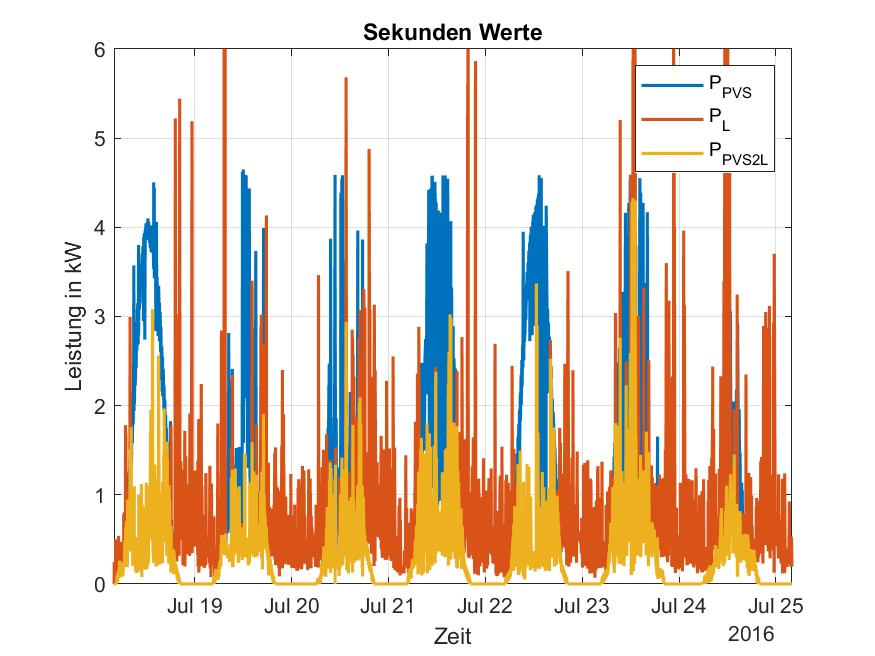
\includegraphics[width=\textwidth]{Abbildungen/plot.jpg}
    \caption{Beschreibung des Plots}
    \label{fig:plot3062023}
\end{figure}
\subsection{2}
$E.E_pvs = sum(ts.Ppvs/1000)/3600=149,96kWh;\\
E.E_l = sum(ts.Pl/1000)/3600=89,08kWh;\\
E.E_pvs2l = sum(Ppvs2l/1000)/3600=41,52kWh;$\\

\subsection{3}
\begin{figure}[H]
    \centering
    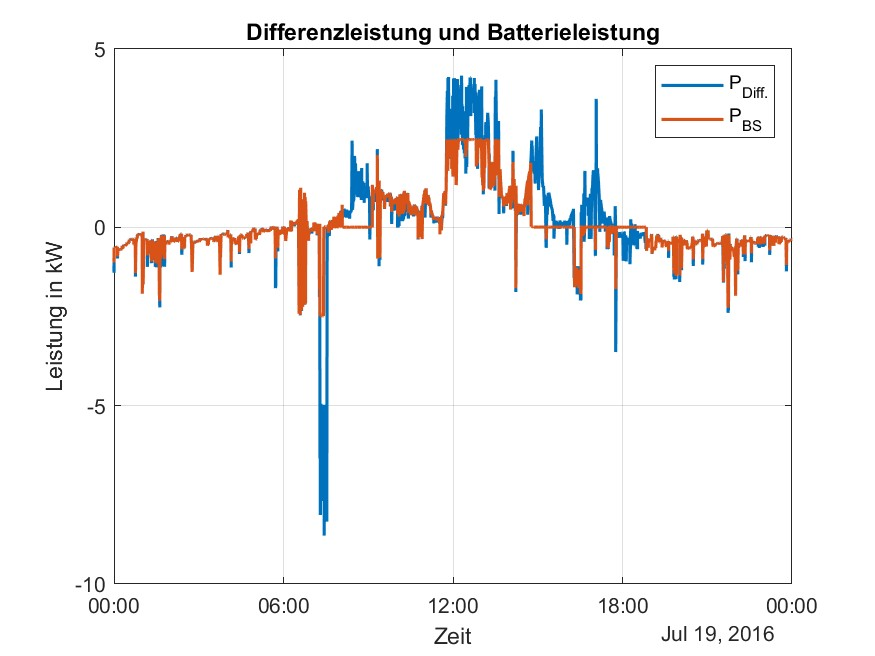
\includegraphics[width=\textwidth]{Abbildungen/plot_vorbereitungsfrage3.jpg}
    \caption{Beschreibung des Plots}
    \label{fig:plot3062023}
\end{figure}
\subsection{4}
\begin{figure}[H]
    \centering
    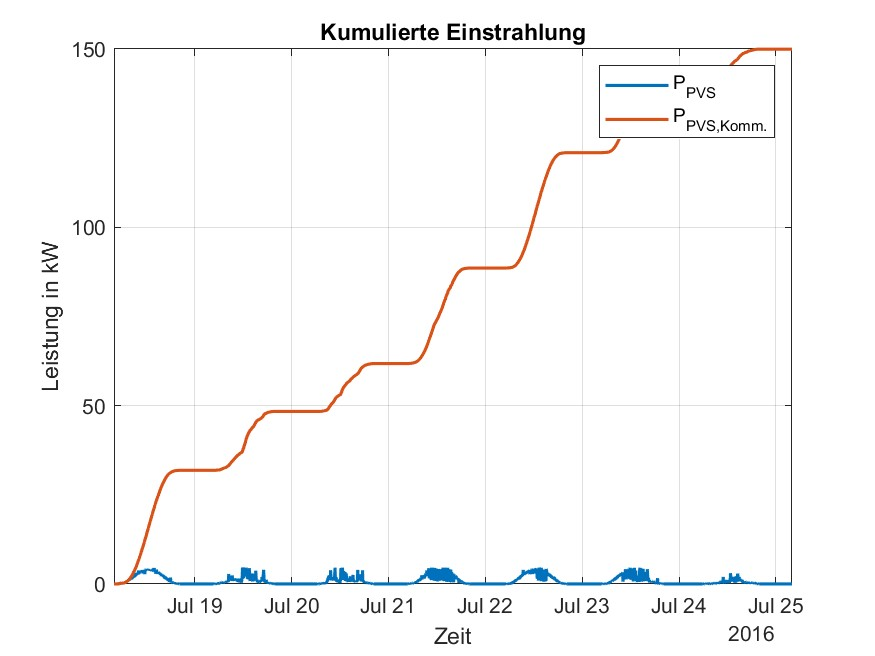
\includegraphics[width=\textwidth]{Abbildungen/plot_vorbereitungsfrage4.jpg}
    \caption{Beschreibung des Plots}
    \label{fig:plot3062023}
\end{figure}
Der MATLAB-Befehl cumsum steht für cumulative sum und wird verwendet, um die kumulative Summe eines Vektors oder einer Matrix zu berechnen. 
Also statt die gesammte Summe zu berechnen, werden mit cumsum auch alle zwischen Summen gespeichert. In \autoref{fig:plot3062023} ist zu sehen, wie mit Hilfe des Befehls die Leistungen kummuliert werden und man eine Aussage über die kummulierte Einstrahlung erhält.